\documentclass[twocolumn,english]{IEEEtran}
\usepackage[T1]{fontenc}
\usepackage{babel}
\usepackage{amsthm}
\usepackage{amsmath}
\usepackage{graphicx}
\usepackage[unicode=true,
bookmarks=true,bookmarksnumbered=true,bookmarksopen=true,bookmarksopenlevel=1,
breaklinks=false,pdfborder={0 0 0},backref=false,colorlinks=false]
{hyperref}
\usepackage{bm}
\usepackage{amsmath}
\usepackage{amssymb}
\usepackage{natbib}
\usepackage{array}
\usepackage{calc}
\newcolumntype{W}{>{\centering\arraybackslash}m{25mm}}
\newcolumntype{L}{>{\centering\arraybackslash}m{15mm}}
\makeatletter
\setcounter{topnumber}{2}
\setcounter{bottomnumber}{2}
\setcounter{totalnumber}{4}
\renewcommand{\topfraction}{0.85}
\renewcommand{\bottomfraction}{0.85}
\renewcommand{\textfraction}{0.15}
\renewcommand{\floatpagefraction}{0.7}
\usepackage{float}
\usepackage{booktabs}

\hypersetup{
pdftitle=  {Lab 4: Diode Circuits},
pdfauthor= {Alex Landry, Nolan Guettler, Zack Garza}%TODO: Fill in names
pdfpagelayout=OneColumn, pdfnewwindow=true, pdfstartview=XYZ, plainpages=false}

\begin{document}

\title{Lab 4: Diode Circuits}
\author{Alex Landry, Nolan Guettler, Zack Garza} %TODO: Fill in names
\IEEEspecialpapernotice{Engineering 17L \\ Effective Date of Report: \today}

\markboth{Lab 4: Diode Circuits}{Zack Garza}
\maketitle

\begin{abstract}
This is some text to fill up the abstract.
\end{abstract}

\tableofcontents

\section{Introduction}
\IEEEPARstart{T}{his} is some placeholder text to make the formatting less wonky.
\subsection{Purpose}

\section{Theory}
%TODO: Explanation of Clippers, Clampers, V regulators, Diodes, Zener Diodes, Logic Gates

\section{Methodology}
\subsection{Equipment List}
\begin{enumerate}
  \item Breadboard
  \item \underline {Measuring Equipment:}
    \begin{enumerate}
      \item Digital Oscilloscope
      \item Digital Multi-Meter \hfill[x2]
    \end{enumerate}
  \item \underline {Power Sources:}
    \begin{enumerate}
    \item DC Power Supply
    \item Function Generator
    \end{enumerate}
  \item \underline{Resistors:}
    \begin{enumerate}
    \item 1.0 k$\Omega$ (1/4 W) \hfill[x1]
    \item 10.0 k$\Omega$ (1/2 W) \hfill[x1]
    \item Variable Resistor Box
    \end{enumerate}
  \item \underline{Diodes:}
    \begin{enumerate}
     \item 1N4002 Diode \hfill[x2]
     \item 1N4737 Zener Diode \hfill[x1]
    \end{enumerate}
  \item \underline{Capacitors:}
    \begin{enumerate}
     \item 0.1 $\mu$F \hfill[x1]
     \item 1.0 $\mu$F (Electrolytic) \hfill[x1]
    \end{enumerate}
\end{enumerate}

\subsection{Diodes as Clippers}
  %TODO: Add two circuit diagrams
  \begin{enumerate}
    \item The circuit was built on the protoboard with $R_1=10$ k$\Omega$. %TODO: Need ref to diagram
    \item The oscilloscope was set to DC coupling mode, and Channels 1 and 2 were displayed simultaneously.
    \item A \textbf{1 kHz triangle wave} was used as the input signal. $V_{s1}$ and $V_{\text{Out 1}}$ were monitored on Channels 1 and 2 respectively.
    \item The following parameters of the input signal were varied, and the effects recorded:
      \begin{enumerate}
       \item DC Offset
       \item Frequency
       \item Peak-to-Peak Voltage
      \end{enumerate}
    \item Screen captures were generated that indicated the clipping behavior of the circuit.
    \item The second diode was wired parallel to the first to observe the resulting clipping effects. %TODO: Explain with diagram, labels?
    \item The following parameters of the input signal were varied, and the effects recorded:
      \begin{enumerate}
       \item DC Offset
       \item Amplitude
       \item Waveform Type
      \end{enumerate}
  \end{enumerate}

\subsection{Diode Clamping}
  %TODO: Add one circuit diagram
  \begin{enumerate}
   \item The circuit was built on the protoboard with $R_2 = 10$ k$\Omega$. %TODO: Ref to diagram
   \item A \textbf{1kHz sine wave} input signal was used, with the \textbf{DC Offset} set to \textbf{zero}.
   \item The oscilloscope was set to DC coupling mode. %TODO: Explain why DC coupling in results
   \item The oscilloscope was then wired to monitor $V_{s2}$ and $V_{\text{Out 2}}$.
   \item The input and output signals were measured on Channels 1 and 2 respectively. %TODO: Ref to diagram
   \item The DC Offset of the input signal was varied, and the effects on the output signal were measured and recorded.
  \end{enumerate}

\subsection{Voltage Regulator}
  %TODO: Add circuit diagram
  \begin{enumerate}
   \item The circuit was built on the protoboard. %TODO: Ref to diagram, add exact values?
   \item A 20 V DC power generator was used as the source voltage.
   \item The oscilloscope was wired to measure the load variables $V_L$ and $i_L$.
   \item The resistance $R_L$ was varied, and data points were collected for both $V_L$ and $i_L$.
   \item A plot was generated of the data points as the experiment was conducted in order to determine where more data points were needed.
  \end{enumerate}

\subsection{AC $\rightarrow$ DC Converter} %Rightarrow causes error, but compiles. Only affects autogenerated table of contents in PDF.
  %TODO: Circuit diagram
  \begin{enumerate}
    \item The circuit was built on the protoboard. %TODO: Ref to diagram.
    \item The function generator was set to produce a \textbf{1 kHz sine wave}.
    \item The capacitor was tested for its polarization and connected appropriately.
    \item The oscilloscope was wired to measure $V_s$ and $V_{\text{Out}}$ on Channels 1 and 2 respectively.
    \item The oscilloscope was set to DC coupling on both channels.
    \item The oscilloscope was zeroed before capturing data. %TODO: Recalibrate? Or adjust levels?
    \item The resistance $R_L$ was varied, and the results were recorded.
    \item The voltages were measured with DVMs and recorded. %TODO: Which voltages?
  \end{enumerate}

\subsection{Diode Logic Circuits}
  %TODO: Diagrams for AND & OR gate circuits
  \begin{enumerate}
   \item The circuit for the \textbf{AND} gate was built on the protoboard.
   \item A \textbf{5 V DC} power source was wired into the protoboard.
   \item The oscilloscope was wired to measure $V_{\text{Out}}$.
   \item Different combinations of voltages were applied to the inputs, and the outputs were recorded.
   \item The procedure was repeated for an \textbf{OR} gate.
  \end{enumerate}

\section{Data and Analysis}


\subsection{\textbf{Clipping Circuit}}

\begin{figure}[H]
  \begin{centering}
  \begin{center}
  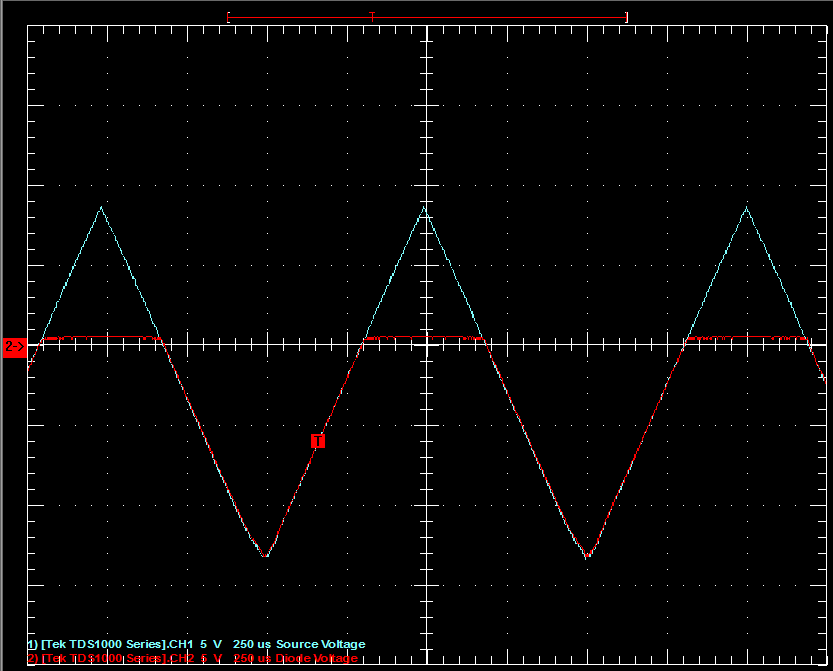
\includegraphics[width=\linewidth]{./Circuit_1.png}
  \caption{Source and diode voltage overlayed to show clipping behavior. The flat portion waveform just above the x-axis represents the clipped output voltage.}
  \label{fig:circuit_1}
  \end{center}
  \par\end{centering}
\end{figure}

As the parameters outlined in the Methodology section were varied, the following observations were made. See Figure~\ref{fig:circuit_1}

\begin{enumerate}

  \item \textit{DC Offset}

    Changing the DC Offset of the signal generator changes the magnitude of the voltage supplied, but does not have a discernible effect on the output voltage. The diode effectively cut off the signal at approximately zero volts, regardless of what voltage was supplied by the source. \\

  \item \textit{Frequency}

    Changing the frequency of the source signal changes the edge behavior of the output voltage slightly.
    At low frequencies, the waveform of the output signal will mirror the input signal, with all voltages above zero rounded down to zero, which effectively flattens out the peaks.
    At higher frequencies, the source and output voltages begin to slip out of phase, and the waveform becomes sinusoidal with a peak at zero volts. \\

  \item \textit{Signal Amplitude}

    Increasing the amplitude of the source signal increases the steepness of the waveform of the output voltage, but does not have a large effect on the clipping behavior.
\end{enumerate}

It was found that the circuit deviates slightly from an ideal clipping circuit. While the theoretical maximum output voltage should be clipped to zero volts, the actual maximum output voltage was measured to be \textbf{552 mV}, which is shown in Figure~\ref{fig:cutoff_voltage}.

\begin{figure}[H]
  \begin{centering}
  \begin{center}
  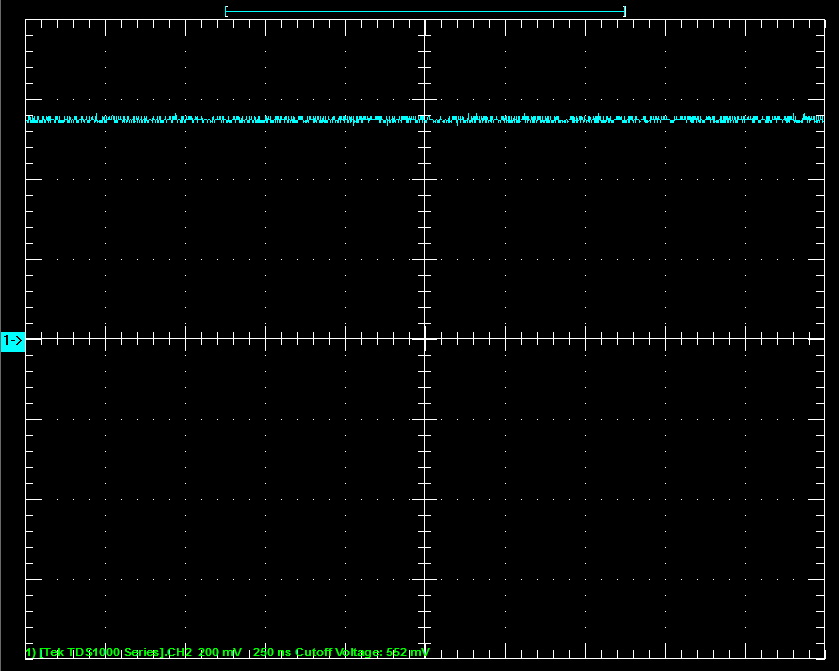
\includegraphics[width=\linewidth]{./Cutoff_Voltage.png}
  \caption{Deviation of cutoff voltage from theoretical ideal of zero volts.}
  \label{fig:cutoff_voltage}
  \end{center}
  \par\end{centering}
  \end{figure}





\subsection{\textbf{Clamping Circuit}}





\subsection{\textbf{Voltage Regulator}}

\begin{figure}[H]
  \begin{centering}
  \begin{center}
  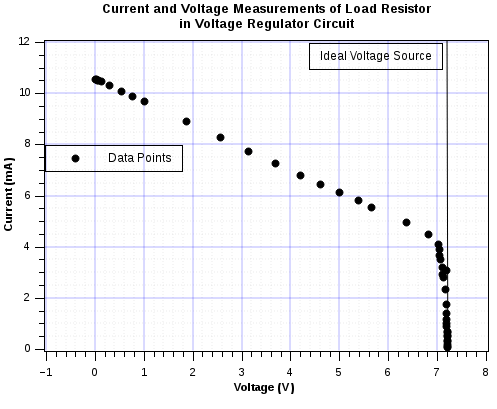
\includegraphics[width=\linewidth]{./voltage_reg.png}
  \caption{Plots of the load resistor's current and voltage, and its deviation from the behavior of an ideal voltage source.}
  \label{fig:voltage_reg}
  \end{center}
  \par\end{centering}
  \end{figure}






\subsection{\textbf{AC $\rightarrow$ DC Converter}}

\begin{figure}[H]
  \begin{centering}
  \begin{center}
  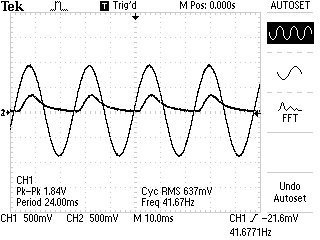
\includegraphics[width=\linewidth]{./DC1.png}
  \caption{Display of input and output signals. The output voltage is not strictly constant, as it exhibits an exponential voltage decay due to the capacitor.}
  \label{fig:DC1}
  \end{center}
  \par\end{centering}
\end{figure}

\begin{figure}[H]
  \begin{centering}
  \begin{center}
  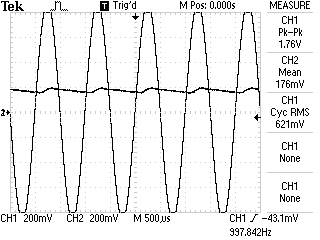
\includegraphics[width=\linewidth]{./DC2.png}
  \caption{As the frequency increases, the voltage drop between cycles decreases.}
  \label{fig:DC2}
  \end{center}
  \par\end{centering}
\end{figure}

\begin{figure}[H]
  \begin{centering}
  \begin{center}
  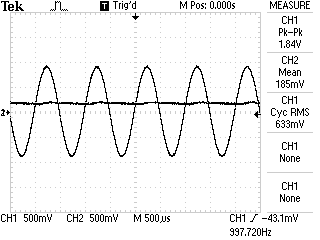
\includegraphics[width=\linewidth]{./DC3_5k.png}
  \caption{Zooming out at a high frequency shows that the output closely approximates a constant DC voltage.}
  \label{fig:DC3}
  \end{center}
  \par\end{centering}
\end{figure}

\begin{figure}[H]
  \begin{centering}
  \begin{center}
  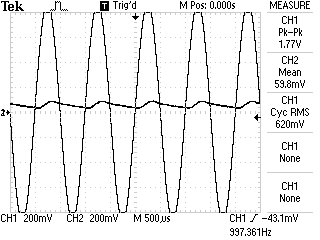
\includegraphics[width=\linewidth]{./DC4_1k.png}
  \caption{Changing the load resistance directly affects the voltage delivered to it. Decreasing the resistance by a factor of 5 lowered the output voltage by a factor of 3.}
  \label{fig:DC4}
  \end{center}
  \par\end{centering}
\end{figure}





\subsection{\textbf{Logic Gates}}

\begin{table}[H]
\centering{}
\caption{AND Gate Truth Table}
\begin{tabular}{@{}ccc@{}}
\toprule
\textbf{Input 1} & \multicolumn{1}{l}{\textbf{Input 2}} & \multicolumn{1}{l}{\textbf{Output}} \\ \midrule
1                & 1                                    & 1                                   \\
1                & 0                                    & 0                                   \\
0                & 1                                    & 0                                   \\
0                & 0                                    & 0                                   \\ \bottomrule
\end{tabular}
\end{table}

\begin{table}[h]
\centering{}
\caption{OR Gate Truth Table}
\begin{tabular}{@{}ccc@{}}
\toprule
\textbf{Input 1} & \multicolumn{1}{l}{\textbf{Input 2}} & \multicolumn{1}{l}{\textbf{Output}} \\ \midrule
1                & 1                                    & 1                                   \\
1                & 0                                    & 1                                   \\
0                & 1                                    & 1                                   \\
0                & 0                                    & 0                                   \\ \bottomrule
\end{tabular}
\end{table}


\appendices{}

%\bibliographystyle{plain}
%\bibliography{physbib}

\end{document}